\subsection{I pacchetti}

Nel mondo delle distribuzioni GNU/Linux, per l'installazione, la rimozione e l'aggiornamento del software si usano dei particolari file binari (solitamente compressi), che prendono il nome di packages (pacchetti).

Nel corso dello sviluppo delle varie distribuzioni, i vari team di sviluppo hanno scelto di differenziare molto, sia per tipologia di pacchetto (rpm, deb, tgz...) sia per gestore di pacchetti (rpm, dpkg, pkgtool...).

Di fatto, ad oggi, non esiste uno standard valido per qualsiasi distribuzione, anche se molte di queste hanno scelto RPM come soluzione. RPM (Red Hat Package Manager) è utilizzato fra le altre da Red Hat e derivate (Red Hat, Fedora, CentOS...), da SUSE (e derivate) e da Mandriva. Questo rende il pacchetto RPM tra i più diffusi in assoluto. 

L'utilizzo del medesimo pacchetto da parte di distribuzioni differenti non garantisce però che i pacchetti siano compatibili tra loro, e nemmeno l'utilizzo del medesimo front-end. In base alla distribuzione infatti, è possibile vedere dei front-end differenti.

\begin{itemize}
 \item yum: Red Hat Enterpise Linux (5.x o successive), Fedora, CentOS (5.x o successive), Yellow Dog, Oracle Linux
 \item zypper: SUSE Linux Enterpise, openSUSE
 \item urpmi: Mandriva, Mageia
 \item up2date: Red Hat Enterpise Linux (precedenti a 5.x), CentOS (precedenti a 5.x), Oracle Linux
\end{itemize}

Il nome del file di un pacchetto rpm è solitamente così composto:

\begin{verbatim}
 <nome>-<versione>-<build>-<distribuzione>-<architettura>.rpm
\end{verbatim}

\begin{itemize}
 \item Nome: Nome del software
 \item Versione: Versione di rilascio del sorgente da cui è stato ricavato il pacchetto.
 \item Build: Numero di volte che la medesima versione del sorgente è stata compilata
 \item distribuzione (opzionale): in alcuni casi si indica la distribuzione di destinazione (es ``rhel6``)
 \item architettura: Codice che rappresenta l'architettura per cui il pacchetto è stato compilato (es. x86, x86\_64, arm, powerpc etc...)
\end{itemize}

Un pacchetto RPM, oltre ad avere la parte binaria, dispone anche di un ``header'', dove sono contenute alcune informazioni importanti relative al pacchetto. 

I pacchetti RPM, al momento dell'installazione, possono essere verificati attraverso i cosidetti algoritmi di summury (MD5) o attraverso verifica di firma crittografica (GPG). Con tali meccanismi si cerca di correggere eventuali errori di download e di evitare la presenza di pacchetti la cui provenienza non sia certificata. 

\subsubsection{Dipendenze}


\begin{figure}[!ht]
 \centering
 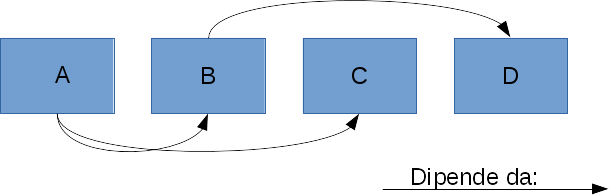
\includegraphics[scale=0.55]{Immagini/dipendenza01.png}
 \label{fig:Dipendenza}
 \caption{Relazione di dipendenza}
\end{figure}

Con i gestori di pacchetti moderni è stato introdotto il concetto di ``dipendenza''. Di fatto, buona parte del software presente in una distribuzione GNU/Linux è in dipendenza di qualche altro software. Una dipendenza è per l'appunto il software necessario ad un altro per funzionare correttamente. 
La verifica delle dipendenze al momento dell'installazione consente di controllare se è presente tutto il software necessario al pacchetto per funzionare. Inoltre, il medesimo processo applicato al momento della rimozione di un pacchetto, evita di andare a rimuovere elemnti utili ad un qualsiasi altro programma. Infine, sempre a mezzo di queste operazioni di verifica, si evita di installare pacchetti in potenziale conflitto fra di loro. 

Le informazioni sui vari pacchetti vengono conservati all'interno di un database di tipo db4 nella cartella \directory{/var/lib/rpm}

\subsection{Il tool rpm}

Il tool rpm, è il comando base da utilizzare per eseguire le varie operazioni sui pacchetti. 

Utilizzato da riga di comando la sua sintassi è

\begin{verbatim}
 # rpm <opzioni> nomepacchetto-versione-build-arch.rpm
 # rpm <opzioni> nomefile
\end{verbatim}

Alcune delle opzioni utilizzabili con rpm

\begin{itemize}
 \item \textbf{-i}: Installare il pacchetto (install)
 \item \textbf{-e}: Rimozione del pacchetto (erase)
 \item \textbf{-U}: Aggiornamento del pacchetto (upgrade)
 \item \textbf{-V}: Verifica del pacchetto installato (verify)
 \item \textbf{-q}: Informazioni sul pacchetto (query)
\end{itemize}

L'opzione ``-q'' offre altre opzioni a cui è abbinabile

\begin{itemize}
 \item \textbf{-qa}: Interroga tutti i pacchetti installati
 \item \textbf{-qf [nomefile]}: Interroga il pacchetto proprietaro del file
 \item \textbf{-qi}: Mosrta le info su un determinato pacchetto
 \item \textbf{-ql}: Mostra l'elenco dei file contenuti nel pacchetto
 \item \textbf{-qs}: Mostra lo stato dei file del pacchetto
 \item \textbf{-qc}: Mostra un elenco dei file di configurazione
\end{itemize}

\subsection{Yum}

Nonostante rpm copra un grande numero di funzioni, nel corso degli anni si sono sviluppati dei front-end per automatizzare alcune operazioni relative all'installazione e all'aggiornamento del sistema. 
Nei sistemi di stretta derivazione Red Hat si utilizza \textbf{yum} (Yellow-dog updater modified); si tratta di un programma, scritto in python che permette di installare, rimuovere, aggiornare e verificare i pacchetti. Inoltre yum, collegandosi a delle particolari locazioni (remote o locali) definite \textbf{``repository''}, scarica il software oggetto di installazione o di aggiornamento e le relative dipendenze. Tutto questo viene fatto in maniera trasparente all'utente.

La sintassi del comando yum è 
\begin{verbatim}
 # yum <opzioni> comando [argomenti]
\end{verbatim}

A seguire alcuni dei comandi eseguibili con yum

\begin{itemize}
 \item \textbf{install} [nomepacchetto]: installa il pacchetto e le relative dipendenze. Accetta argomenti multipli
 \item \textbf{update} [nomepacchetto]: aggiorna il pacchetto selezionato. Senza argomenti aggiorna tutto il sistema.
 \item \textbf{remove} [nomepacchetto]: rimuove il pacchetto, e, se è dipendenza di altri richiede la rimozione.
 \item \textbf{provides} [nomefile]: fornisce il nome del pacchetto che offre il file
 \item \textbf{downgrade} [nomepacchetto]: riporta il pacchetto ad una versione precedente.
 \item \textbf{info} [nomepacchetto]: mostra le informazioni relative al pacchetto
 \item \textbf{check}: Identifica gli errore all'interno del rpmdb
\end{itemize}


I ``repository'' sono definiti all'interno di file di testo, con estensione \textbf{``.repo''}, presenti nella cartella \directory{/etc/yum.repos.d/}.
A seguire un esempio di un file .repo. 

\begin{verbatim}
[base]
name=CentOS-$releasever - Base
baseurl=http://mirror.centos.org/centos/$releasever/os/$basearch/
gpgcheck=1
gpgkey=file:///etc/pki/rpm-gpg/RPM-GPG-KEY-CentOS-6
\end{verbatim}


\subsection{PackageKit}

\begin{figure}[!ht]
  \centering
  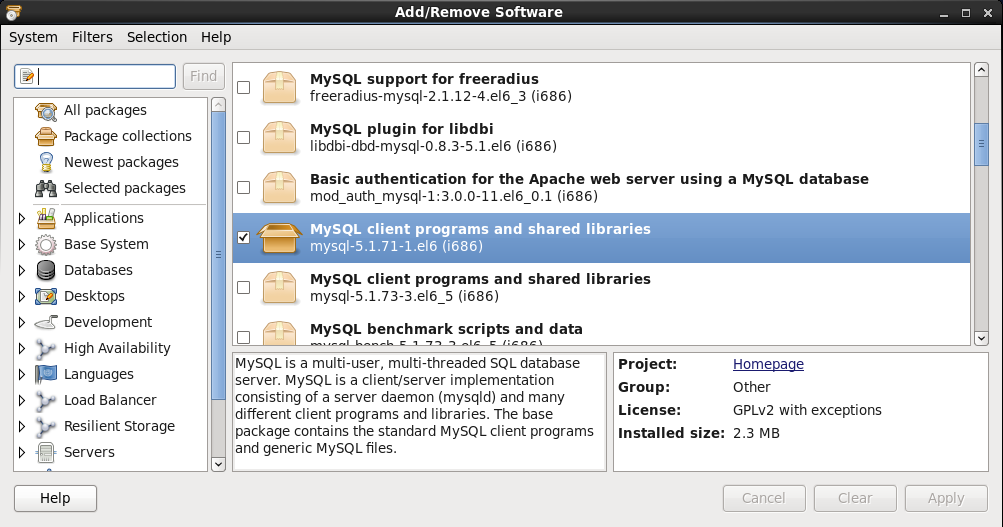
\includegraphics[scale=0.4]{Immagini/packagekit1.png}
  \label{fig:PackageKit}
  \caption{PackageKit front-end}
\end{figure}


Il tool da interfaccia grafica PackageKit, permette, attraverso una serie di menù intuitivi e guidati, di compiere tutte le operazioni relative alla ricerca, download, installazione, aggiornamento o rimozione dei pacchetti. 
PackageKit si basa su yum, ed è reperibile nel menu alla voce \menu{System > Administration > Add/Remove Software}.



